\documentclass[]{tufte-handout}

% ams
\usepackage{amssymb,amsmath}

\usepackage{ifxetex,ifluatex}
\usepackage{fixltx2e} % provides \textsubscript
\ifnum 0\ifxetex 1\fi\ifluatex 1\fi=0 % if pdftex
  \usepackage[T1]{fontenc}
  \usepackage[utf8]{inputenc}
\else % if luatex or xelatex
  \makeatletter
  \@ifpackageloaded{fontspec}{}{\usepackage{fontspec}}
  \makeatother
  \defaultfontfeatures{Ligatures=TeX,Scale=MatchLowercase}
  \makeatletter
  \@ifpackageloaded{soul}{
     \renewcommand\allcapsspacing[1]{{\addfontfeature{LetterSpace=15}#1}}
     \renewcommand\smallcapsspacing[1]{{\addfontfeature{LetterSpace=10}#1}}
   }{}
  \makeatother

\fi

% graphix
\usepackage{graphicx}
\setkeys{Gin}{width=\linewidth,totalheight=\textheight,keepaspectratio}

% booktabs
\usepackage{booktabs}

% url
\usepackage{url}

% hyperref
\usepackage{hyperref}

% units.
\usepackage{units}


\setcounter{secnumdepth}{-1}

% citations


% pandoc syntax highlighting

% table with pandoc

% multiplecol
\usepackage{multicol}

% strikeout
\usepackage[normalem]{ulem}

% morefloats
\usepackage{morefloats}


% tightlist macro required by pandoc >= 1.14
\providecommand{\tightlist}{%
  \setlength{\itemsep}{0pt}\setlength{\parskip}{0pt}}

% title / author / date
\title{Introducción: ¿Qué es R?}
\author{Jorge Meneses \and Paulo Peña}
\date{}


\begin{document}

\maketitle




\begin{verbatim}
## [1] "C:/Users/Paulo/Documents/GitHub/introduccion_R/sesiones/01 - que es R/que es R.Rmd"
\end{verbatim}

\hypertarget{introducciuxf3n}{%
\section{Introducción}\label{introducciuxf3n}}

\begin{itemize}
\tightlist
\item
  Curso práctico: En cada sesión habrán ejercicios a resolver
\item
  Sesiones de 45 minutos
\end{itemize}

\hypertarget{objetivos-del-curso}{%
\subsection{Objetivos del curso}\label{objetivos-del-curso}}

\begin{itemize}
\tightlist
\item
  Conocer la sintaxis básica de R
\item
  Importar y exportar bases de datos
\item
  Elaboración de tablas de frecuencias
\item
  Generación de reportes (Rmarkdown)
\item
  Visualización de datos
\end{itemize}

\hypertarget{quuxe9-es-r}{%
\section{¿Qué es R?}\label{quuxe9-es-r}}

R es un \textbf{lenguaje de programación} de \textbf{código abierto}
ampliamente usado para el análisis de datos y la estadística. Está
disponible para Windows, macOS y Linux.

\begin{itemize}
\tightlist
\item
  \textbf{¿Qué implica un lenguaje de programación?:} Un lenguaje de
  programación son instrucciones dadas a una computadora para dar una
  tarea.
\end{itemize}

\hypertarget{porque-usar-r}{%
\subsection{¿Porque usar R?}\label{porque-usar-r}}

\begin{itemize}
\tightlist
\item
  R es una herramienta líder para la estadística y el análisis de datos.
\item
  Es un lenguaje de programación independiente del sistema operativo.
\item
  Es de código abierto y gratuito.
\item
  Tiene una gran comunidad de usuarios a nivel global.
\item
  Replicabilidad del análisis: La sintaxis guarda los pasos específicos
  hechos para generar un análisis. Otros investigadores pueden verificar
  o replicar los estudios.
\end{itemize}

\hypertarget{rstudio}{%
\subsection{Rstudio}\label{rstudio}}

\begin{marginfigure}
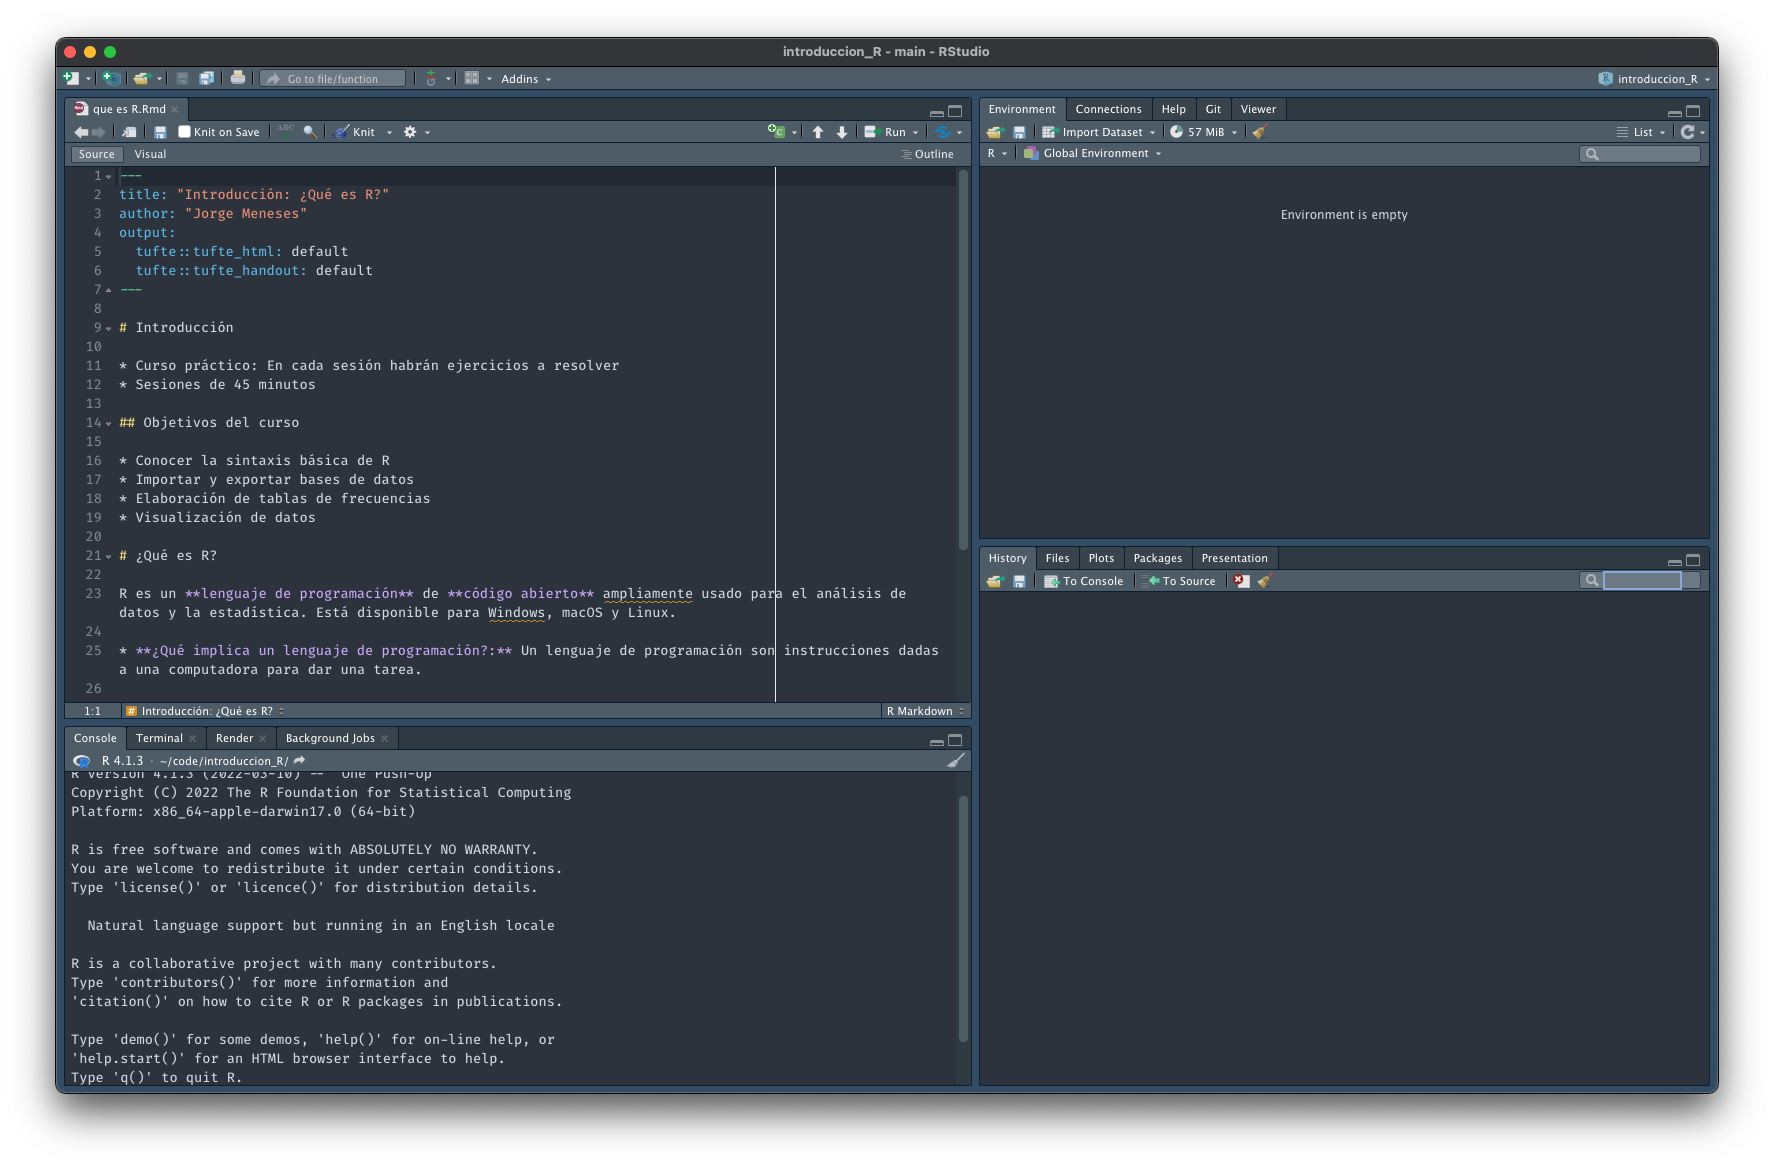
\includegraphics[width=24.64in]{../../public/img/01 - Rstudio} \caption[Rstudio]{Rstudio}\label{fig:unnamed-chunk-2}
\end{marginfigure}

Rstudio es la aplicación más usada para desarrollar R. Es lo que se
conoce como un \textbf{IDE} (Integrated Development Environment, o
Entorno de Desarrollo Integrado). Esta aplicación esta diseñada para
facilitar el desarrollo de análisis y reportes en R.

\hypertarget{instalar-r-y-rstudio}{%
\section{Instalar R y Rstudio}\label{instalar-r-y-rstudio}}

Para seguir con el curso práctico requerimos la instalación de R y
Rstudio en nuestras computadoras. La instalación dependerá del sistema
operativo que usemos

\hypertarget{instalar-r-y-rstudio-en-windows}{%
\subsection{Instalar R y Rstudio en
Windows}\label{instalar-r-y-rstudio-en-windows}}

\textbf{Descargar e instalar R}

\textbf{Descargar e instalar Rstudio}

\hypertarget{instalar-r-y-rstudio-en-macos}{%
\subsection{Instalar R y Rstudio en
macOS}\label{instalar-r-y-rstudio-en-macos}}

\textbf{Descargar e instalar R}

\textbf{Descargar e instalar Rstudio}



\end{document}
